\documentclass[10pt]{article}

% Specify the margins and text size.
\setlength{\textwidth}{6.4in}
\setlength{\textheight}{9.5in}
\setlength{\oddsidemargin}{0pt}
\setlength{\evensidemargin}{0pt}
\setlength{\topmargin}{0pt}
\setlength{\hoffset}{.05in}
\setlength{\voffset}{-1in}

\setlength{\parskip}{5pt}
\setlength{\parindent}{0pt}

% Load some fonts and symbol packages
\usepackage{latexsym}
\usepackage{pifont}       % contains 'star' symbol for counterinsurgency handbook title
\usepackage{yfonts} 
\usepackage{amsmath}
\usepackage{amsfonts}

\usepackage{graphicx}     % actually, this is loaded by pstricks
\usepackage[T1]{fontenc}
\usepackage{ifthen}
\usepackage{pstricks,pst-grad,pst-text,pst-node,multido,pst-plot,calc,pst-3dplot}
%\usepackage[all]{xy}
%\usepackage{animate}

% The hyperref package inserts links into the pdf.
\definecolor{MyLinkColor}{rgb}{.1,.2,1}
\definecolor{MyCiteColor}{rgb}{.1,1,.2}
\definecolor{MyURLColor}{rgb}{.4,.4,.4}
\usepackage[backref=true,pagebackref=false,hyperindex,colorlinks=true,
  linkcolor=MyLinkColor,urlcolor=MyURLColor]{hyperref}


% The tweaklist package is something I found on the web.  It provides a simple interface
% for making changes to spacing used in the itemize and enumerate environments.  Comment
% this out if you don't care to use tweaklist.
\usepackage{tweaklist}
\renewcommand{\itemhook}{\setlength{\parskip}{2pt}\setlength{\parsep}%
{1pt}\setlength{\topsep}{0pt}\setlength{\itemsep}{0pt}}

\newcommand{\U}{\underline{\hspace{5pt}}}

\usepackage{listings}
\newcounter{EX}\setcounter{EX}{1}
\newcommand{\EXERCISE}{\arabic{EX}.\stepcounter{EX} }

\begin{document}
\pagestyle{empty}
\lstset{language=R, showspaces=false, showstringspaces=false}

\href{http://www.su.edu}{
\includegraphics[height=1.75cm]{sulogo.eps}}
\vspace{-1.69cm}

{\small
\begin{tabular}{cl}
& Math 207\\ & Introduction to  Statistics\\
\hspace{5in} & %18 January 2012
\end{tabular}
}
\setlength{\baselineskip}{1.05\baselineskip}
\bigskip

\begin{center}
\textbf{\large  Using \texttt{R} to Plot Histograms (II)}
\end{center}
\medskip

The \texttt{barplot} and \texttt{hist} commands in \texttt{R} can be used
to plot histograms.  The latter is used when the raw data is available.
\texttt{barplot} is used when we already have the data organized into 
a table.
\medskip

\newcommand{\SUBX}{\smallskip\hspace{10pt}}
\newcommand{\BSK}{\vspace{.14in}}

\EXERCISE 
The distribution of families by income in the U.S. in 1973 is tabulated below.
\begin{center}
\begin{tabular}{cr}
Income level & Percent\\\hline
\$0--\$1,000 & 1\vphantom{\LARGE Y}\\
\$1,000--\$2,000 & 2\\
\$2,000--\$3,000 & 3\\
\$3,000--\$4,000 & 4\\
\$4,000--\$5,000 & 5\\
\$5,000--\$5,000 & 5\\
\$6,000--\$7,000 & 5\\
\$7,000--\$10,000 & 15\\
\$10,000--\$15,000 & 26\\
\$15,000--\$25,000 & 26\\
\$25,000--\$50,000 & 8\\
\$50,000 and over  & 1
\end{tabular}
\end{center}
The percentages give the areas of the boxes of a histogram.  The class
intervals (income level intervals) give the widths.
\texttt{ > incomePercents <- c(1,2,3,4,5,5,5,15,26,26,8)}\par
Let's enter the widths (in units of 
thousands of dollars) of the class intervals.\par
\texttt{ > intervalWidths <- c(1,1,1,1,1,1,1,3,5,10,25)}\par
The heights of the boxes in the histogram should be measured in
   \lq percent per thousand dollars\rq\ so that areas are percentages.  
We compute these by dividing the percent 
  by the width of the corresponding
  class interval.  We  do this as one (vector) step in the first argument 
  to \texttt{barplot} below.\par
\texttt{ > barplot(incomePercents/intervalWidths, intervalWidths, space=0,}\\ 
{\hbox{\hspace{15pt}}}\texttt{  xlab="Income (thousands of dollars)", ylab="Percent per Thousand Dollars", cex.axis=.75)}\\
\texttt{ > axis(1, seq(0,50,by=5), cex.axis=0.75)}\par
The output produced is shown below in Figure~\ref{fig:incomes}.  
Let's describe the parameters passed to \texttt{barplot}.

\begin{tabular}{cll}
$\bullet$ &  \texttt{incomePercents/intervalWidths} & heights of the boxes\\
$\bullet$ &  \texttt{intervalWidths} & widths of the class intervals\\
$\bullet$ &  \texttt{space=0}        & space (none) included between the bars\\
$\bullet$ &  \texttt{xlab="Income (thousands of dollars)"} &  label to put below the x axis\\
$\bullet$ &  \texttt{ylab="Percent per Thousand Dollars"}  &  label to put left of the y axis\\
$\bullet$ &  \texttt{cex.axis=.75}   & reduce the size of numbers along the axes by 25\%\\
\end{tabular}

After we use \texttt{barplot}, we use the \texttt{axis} command to put a income measurements
along the x-axis.  The parameters passed to \texttt{axis} are described below.

\begin{tabular}{cll}
$\bullet$ &  \texttt{1} & apply this to the x-axis\\
$\bullet$ &  \texttt{seq(0,50,by=5)} & put tick marks from 0 to 50 in intervals of 5 units\\
$\bullet$ &  \texttt{cex.axis=.75}   & reduce the size of numbers along the axes by 25\%\\
\end{tabular}
\vfill
\eject

\begin{figure}[h]
\begin{center}
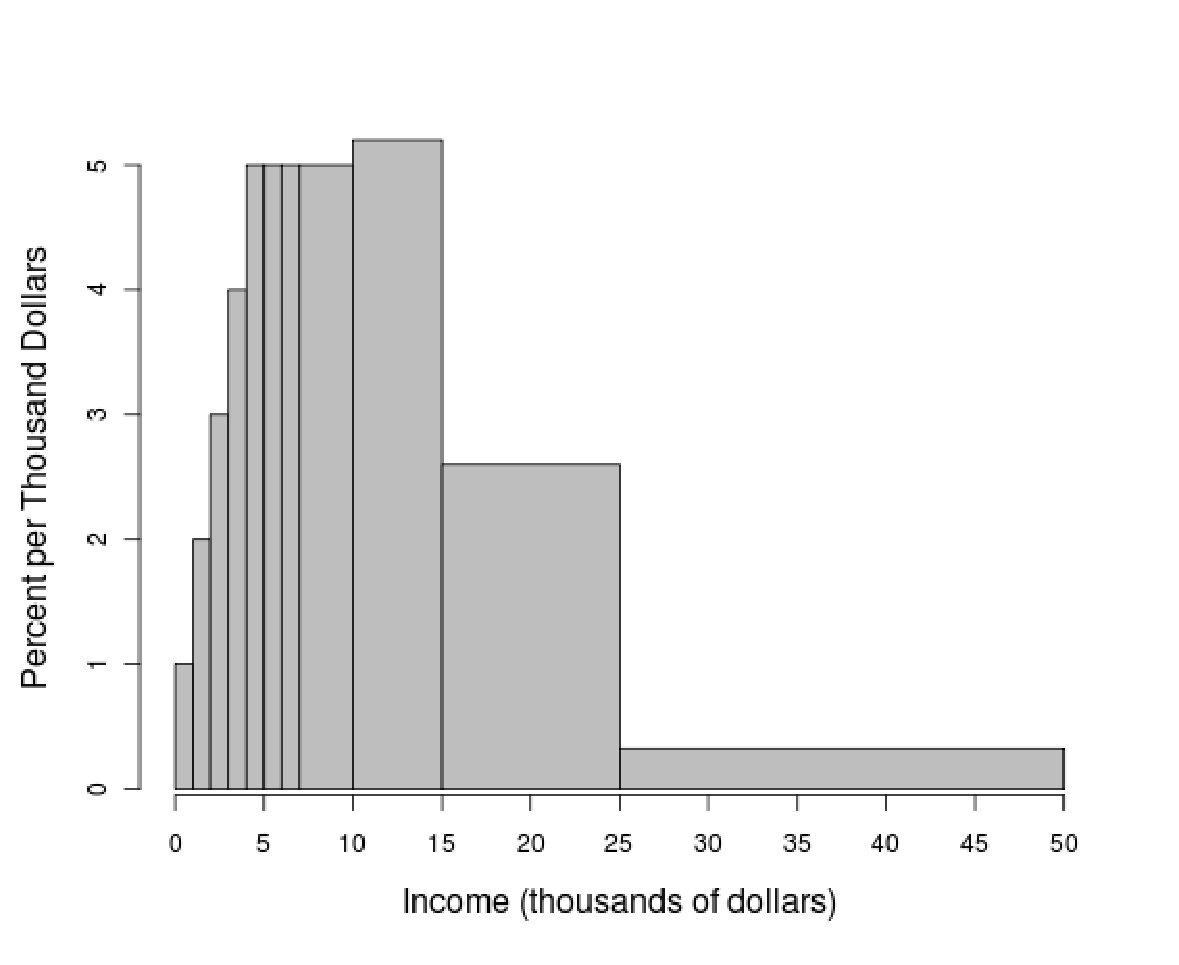
\includegraphics[height=2.9in, bb=0 16 550 380, clip]{Fig4p37.eps}
\caption{\label{fig:incomes}Family income distribution histogram from Figure~4 on page~37 of our text}\vspace{-1in}
\end{center}
\end{figure}
\vspace{1in}

\EXERCISE The table below gives the distribution of educational level 
for persons age 25 and over  in the U.S. in 1960, 1970 and 1971.  \vspace{-10pt}
\begin{center}
\begin{tabular}{crrr}
Educational level \\
(years of schooling) & 1960 & 1970 & 1991\\
0--5 & 8 & 6 & 2\\
5--8 & 14 & 10 & 4\\
8--9 & 18 & 13 & 4\\
9--12 & 19 & 19 & 11\\
12--13 & 25 & 31 & 39\\
13--16 & 9 & 11 & 18\\
16 or more & 8 & 11 & 21
\end{tabular}
\end{center}

\renewcommand{\U}{\underline{\hspace{10pt}}}


\SUBX a) Make a histogram
for the 1960 data.

\texttt{ > educationLevels <- c(2, 4, }\U, \U, \U, \U, \U)\par
\texttt{ > intervalWidths  <- c(5, 3, }\U, \U, \U, \U, 1)\par
\texttt{ > barplot(educationLevels/intervalWidths, } \U\U\U\U\U\U\ %
    \texttt{, space=0,}\\ 
{\hbox{\hspace{15pt}}}\texttt{ xlab="Education Level (years)", ylab="Percent per} \U\U\U
   \texttt{", cex.axis=.75)}\par
\texttt{ > axis(1, seq(0,17,by=1), cex.axis=0.75)}\par
\medskip

\SUBX b) Repeat a) for the 1970 and 1991 data.

\SUBX c) Discuss any interesting
features that you see in the histograms.



\vfill
\eject

\end{document}


Use the Export command on the plot tab in R Studio to produce a jpg file with your plot.
\bigskip

\EXERCISE Use \texttt{R} to do Exercise 2 from page 38 of our text. 
\medskip

\EXERCISE Do Exercise 3 from page 38 of our text. 


